\documentclass[sort&compress,final,numberedheadings]{aipproc}

\layoutstyle{8x11single}

\begin{document}

\title{Nuclear thermodynamics below particle threshold}

\classification{05.20.Gg, 05.70.Fh, 21.10.Ma, 24.10.Pa}

\keywords{Nuclear level density, phase transitions, thermal models, ensemble 
theory}

\author{A.~Schiller}{
address={National Superconducting Cyclotron Laboratory, Michigan State 
University, East Lansing, MI, 48824}
}

\author{U.~Agvaanluvsan}{
address={Lawrence Livermore National Laboratory, L-414, 7000 East Avenue, 
Livermore, CA, 94551},
altaddress={North Carolina State University, Raleigh, NC, 27695}
}

\author{E.~Algin$^{\scriptscriptstyle **,}$}{
address={Department of Physics, Osmangazi University, Meselik, Eskisehir, 26480
Turkey},
altaddress={North Carolina State University, Raleigh, NC, 27695},
altaddress={Triangle Universities Nuclear Laboratory, Durham, NC, 27708}, 
}

\author{A.~Bagheri}{
address={Department of Physics, University of Oslo, N-0316 Oslo, Norway}
}

\author{R.~Chankova}{
address={Department of Physics, University of Oslo, N-0316 Oslo, Norway}
}

\author{M.~Guttormsen}{
address={Department of Physics, University of Oslo, N-0316 Oslo, Norway}
}

\author{M.~Hjorth-Jensen}{
address={Department of Physics, University of Oslo, N-0316 Oslo, Norway}
}

\author{J.~Rekstad}{
address={Department of Physics, University of Oslo, N-0316 Oslo, Norway}
}

\author{S.~Siem}{
address={Department of Physics, University of Oslo, N-0316 Oslo, Norway}
}

\author{A.C.~Sunde}{
address={Department of Physics, University of Oslo, N-0316 Oslo, Norway}
}

\author{A.~Voinov}{
address={Department of Physics and Astronomy, Ohio University, Athens, OH, 
45701}
}

\begin{abstract}
From a starting point of experimentally measured nuclear level densities, we 
discuss thermodynamical properties of nuclei below the particle emission 
threshold. Since nuclei are essentially mesoscopic systems, a straightforward 
generalization of macroscopic ensemble theory often yields unphysical results.
A careful critique of traditional thermodynamical concepts reveals problems 
commonly encountered in mesoscopic systems. One of which is the fact that 
microcanonical and canonical ensemble theory yield different results, another 
concerns the introduction of temperature for small, closed systems. Finally, 
the concept of phase transitions is investigated for mesoscopic systems.
\end{abstract}

\maketitle

\section{Introduction}

Statistical physics and thermodynamics are theories formulated in the 
thermodynamical limit, i.e., for large particle numbers $N\rightarrow\infty$. 
Generalizing those theories to mesoscopic systems like, e.g., atomic nuclei, is
an area of active research as can be seen by several other contributions to 
this book. In subatomic physics, thermodynamical concepts have been employed 
among others in the discussion of the quark-gluon plasma \cite{MH00} and the 
liquid-gas phase transition \cite{PM95}. Fruitful applications of 
thermodynamical concepts in low-energy nuclear physics are the description of 
particle evaporation spectra \cite{Er60} and several other 
temperature-dependent nuclear properties like, e.g., nuclear shapes, giant 
dipole resonance widths, and their fluctuation properties \cite{KA98}. More 
recently, the transition from nucleon pairs coupled to spin $S=0$ and isospin 
$T=1$ at low or zero temperature (Cooper pairs), to an unpaired nucleus at 
higher temperatures has been found experimentally \cite{MB99} and is the 
subject of the present work. Within nuclear theory, temperature-dependent 
calculations have been performed by essentially replacing the particle-number 
operator by its temperature-dependent expectation value (the Fermi-Dirac 
distribution) \cite{SW72}, or by directly using the canonical or 
grand-canonical ensemble theory to calculate thermal expectation values and 
their fluctuations \cite{KA98}. One example, the shell-model Monte Carlo method
is discussed in the contribution by Y. Alhassid to this book. 

\section{Nuclear level densities}

The starting point for all discussions in this work are experimentally measured
nuclear level densities. Unfortunately, space will not permit a thorough 
discussion of the experimental method. In typical experiments, a nucleus is 
heated by a $(^3$He$,\alpha)$ transfer reaction with a beam energy of 
$\sim 45$~MeV\@. At $45^\circ$, this reaction is dominated by high $l$ neutron 
transfer into one-particle-one-hole components of the nuclear wavefunction. For
energies of the residual nucleus above $\sim 2$--4~MeV in the case of 
rare-earth nuclei such configurations are not eigenstates of the nucleus and 
the reaction becomes fairly unselective \cite{RN84}. Thus, we can assume that 
all levels within the spin window of 2--8~$\hbar$ will be populated to some 
degree. If the energy of the residual nucleus $E_i$ (determined by reaction 
kinematics and $Q$ value) is above this energy and below the particle (neutron)
separation energy of 6--8~MeV, the by far dominating decay channel ($\gg 99$\%)
will be statistical $\gamma$ decay. The Brink-Axel hypothesis \cite{Br55+Ax62} 
assumes that statistical $\gamma$ decay can be completely described by the 
so-called $\gamma$-transmission coefficient ${\cal{T}}(E_\gamma)$ (which is 
dependent only on the $\gamma$ transition energy $E_\gamma$), and by the level 
density of final states $\rho(E_f)$ (at energies $E_f=E_i-E_\gamma$). Thus, 
from a collection of unfolded (i.e., corrected for partial energy deposition in
the detector \cite{GT96}), first-generation (i.e., corrected for 
second-and-higher generation $\gamma$ rays in a $\gamma$-ray cascade 
\cite{GR87}) $\gamma$ spectra from different excitation energies $E_i$, one can
obtain simultaneously a model-independent nuclear level density and 
$\gamma$-transmission coefficient \cite{HB95,SB00}. Three independent 
observables from outside of the present experiment (the number of discrete 
levels at very low energy, the average spacing of neutron resonances, and the 
average radiative width of neutron resonances) are used to bring the 
experimental nuclear level density and $\gamma$-transmission coefficient to an 
absolute scale and to fix an ambiguity in the common slope of the two 
functions. The experimental method has been introduced as sequential extraction
method some thirty years ago \cite{BA73} but is also called Oslo method, since 
recently, it has been fully implemented and explored by a group at the Oslo 
Cyclotron Laboratory, Norway. The new information which is provided by the Oslo
method is an interpolation (independent of any functional form) of the nuclear 
level density between the two known points (i) at very low energies (from 
counting of discrete levels) and (ii) at the neutron separation energy (from 
neutron resonance spacing) \cite{MG01,SG02,GM03,SA03,GB03,AS04}. The method 
also provides an extrapolation (again independent of any functional form) of 
the total $\gamma$-transmission coefficient (or the related total radiative 
strength function) from the value obtained by total or partial average 
radiative widths of neutron resonances down to $\gamma$ energies of 1--2~MeV 
\cite{MG01,SG02,GM03,GB03,AS04,VG01,VA04}. The results on radiative strength 
functions will not be discussed further in the present work. Figure 
\ref{fig:dyyb} shows examples of experimental level densities for 
$^{160-162}$Dy \cite{GB03} and $^{170-172}$Yb \cite{AS04}. Other published data
are available for $^{56,57}$Fe and $^{96,97}$Mo \cite{SA03}, $^{166,167}$Er 
\cite{MG01}, $^{148,149}$Sm \cite{SG02}, and $^{27,28}$Si \cite{GM03}. The data
on $^{28}$Si are of special interest for the validation of the Oslo method, 
since all levels up to the particle separation energy (including their spins, 
parities, lifetimes and branching ratios) are known from discrete spectroscopy,
such that the level density and radiative strength function obtained by the 
Oslo method can be compared at all energies to corresponding values derived 
from literature. 

Besides these published data, investigations are ongoing for different Sc, V, 
Ti, Mo, Sn, Sm, and Pb nuclei.

\begin{figure}
\includegraphics[totalheight=10cm,angle=0,bb=107 31 481 783,clip]{fig1a.ps}
\hspace*{2cm}
\includegraphics[totalheight=10cm,angle=0,bb=107 31 481 783,clip]{fig1b.ps}
\caption{Experimental level densities for Dy (left panel) \protect\cite{GB03}, 
and Yb (right panel) isotopes \protect\cite{AS04}. Full data points denote data
from the $(^3$He$,\alpha)$ reaction, open data points are from the 
$(^3$He,$^3$He$^\prime)$ reaction. Those two reactions performed on different 
target nuclei (but resulting in the same residual nucleus) yield very similar 
results. This gives confidence in the Oslo method. The reason for the 
disagreement between the two reactions (mostly for even residual nuclei like 
$^{162}$Dy and $^{172}$Yb) at very low energies (below 1 MeV) has been 
discussed in detail in Ref.\ \protect\cite{SG00}.}
\label{fig:dyyb}
\end{figure}

\subsection{Fine structure in level density}

One of the most attractive features of the Oslo method is that it interpolates 
the level density between $\sim 2$ and $\sim 7$~MeV without assuming any 
functional form. This enables us to observe fine structures in the level 
density \cite{TB95,MB99}. These fine structures are thought to reflect the 
breaking of individual pairs. A simple single-particle plus pairing model is 
able to qualitatively explain the emergence of such fine 
structures.\footnote{Collectivity in nuclei like vibrations and rotations is 
able to create a visible enhancement in the number of levels below the pairing
gap. Compared to the explosion of the number of levels caused by the breaking 
of just one single nucleon pair, however, collective enhancements of the level
density are negligible and are most often not taken into account in our work.}
The model assumes a number $N$ of equally-spaced $\epsilon$, doubly-degenerate 
single-particle levels. Two particles in the same single-particle orbital 
experience the attractive interaction $G$. The Hamiltonian for this problem is
\begin{equation}
{\cal{H}}=\epsilon\,\sum_{\lambda=1}^N\,\lambda\,a_\lambda^\dagger\,a_\lambda\,
-\,G\,\sum_{\mu,\nu=1}^N\,a_\mu^\dagger\,a_{\bar{\mu}}^\dagger\,
a_{\bar{\nu}}\,a_\nu.
\end{equation}
The parameter $\epsilon$ sets the overall energy scale, the parameter 
$\delta=\epsilon/G$ is the only 'intrinsic' parameter of the problem. It is 
the ratio between the spacing of single-particle levels and the attractive 
pairing interaction. For a small number of particles ($\sim 12$) in a small 
number of doubly-degenerate single-particle levels ($N\sim 12$), this problem
can be solved for all eigenvalues \cite{GB00}. For a realistic value of 
$\delta$ in the order of 0.5, the eigenvalues cluster roughly at energies of 
$+{\cal{S}}\,\Delta$ above the ground state, where $\cal{S}$ is the prevalent 
seniority quantum number, i.e., the number of unpaired particles for 
eigenstates at this energy and $\Delta$ is the pairing gap (determined by the
gap equation). Bumps with higher prevalent seniority numbers contain 
progressively more states, since there are more possibilities to distribute two
unpaired particles than one Cooper pair of particles on the single-particle 
level scheme until the model space becomes exhausted. It has been shown that 
smoothing of the seniority bumps (either by a Gaussian smoothing of the 
eigenvalue distribution as in Ref.\ \cite{GB00} or by introducing a seniority 
non-conserving interaction in the Hamiltonian as in Ref.\ \cite{SA03}), the 
gaps between the seniority bumps will be filled and become plateaus, while the 
seniority bumps themselves are degraded to step structures between the 
plateaus. This is illustrated in Fig.\ \ref{fig:femotheo}. Thus, schematic 
microscopic calculations support our claim that step structures in the level 
density curves are signs of breaking of consecutive pairs. Also, what can be 
investigated is how pairing correlations on the one hand are weakened in the 
presence of already unpaired nucleons and how on the other hand those unpaired 
nucleons around the Fermi energy due to the blocking effect of the Pauli 
principle can increase the cost in energy to break up further nucleon pairs. 
This competition is relevant for the pair breaking process in odd nuclei and 
the breaking of the second and higher pairs in even-even nuclei. It is now 
interesting to investigate how the process of pair breaking in a mesoscopic 
system like the atomic nucleus can be cast into the language of thermodynamics,
which has been very successful in describing the transition of other paired 
Fermionic systems like superconductors or superfluid $^3$He to their respective
unpaired, normal phases. This will be the subject of the present work. Many 
aspects of this subject are reviewed by D. J. Dean and M. Hjorth-Jensen in 
Ref.\ \cite{DJ03}.

\begin{figure}
\includegraphics[height=5cm]{fig2a.eps}
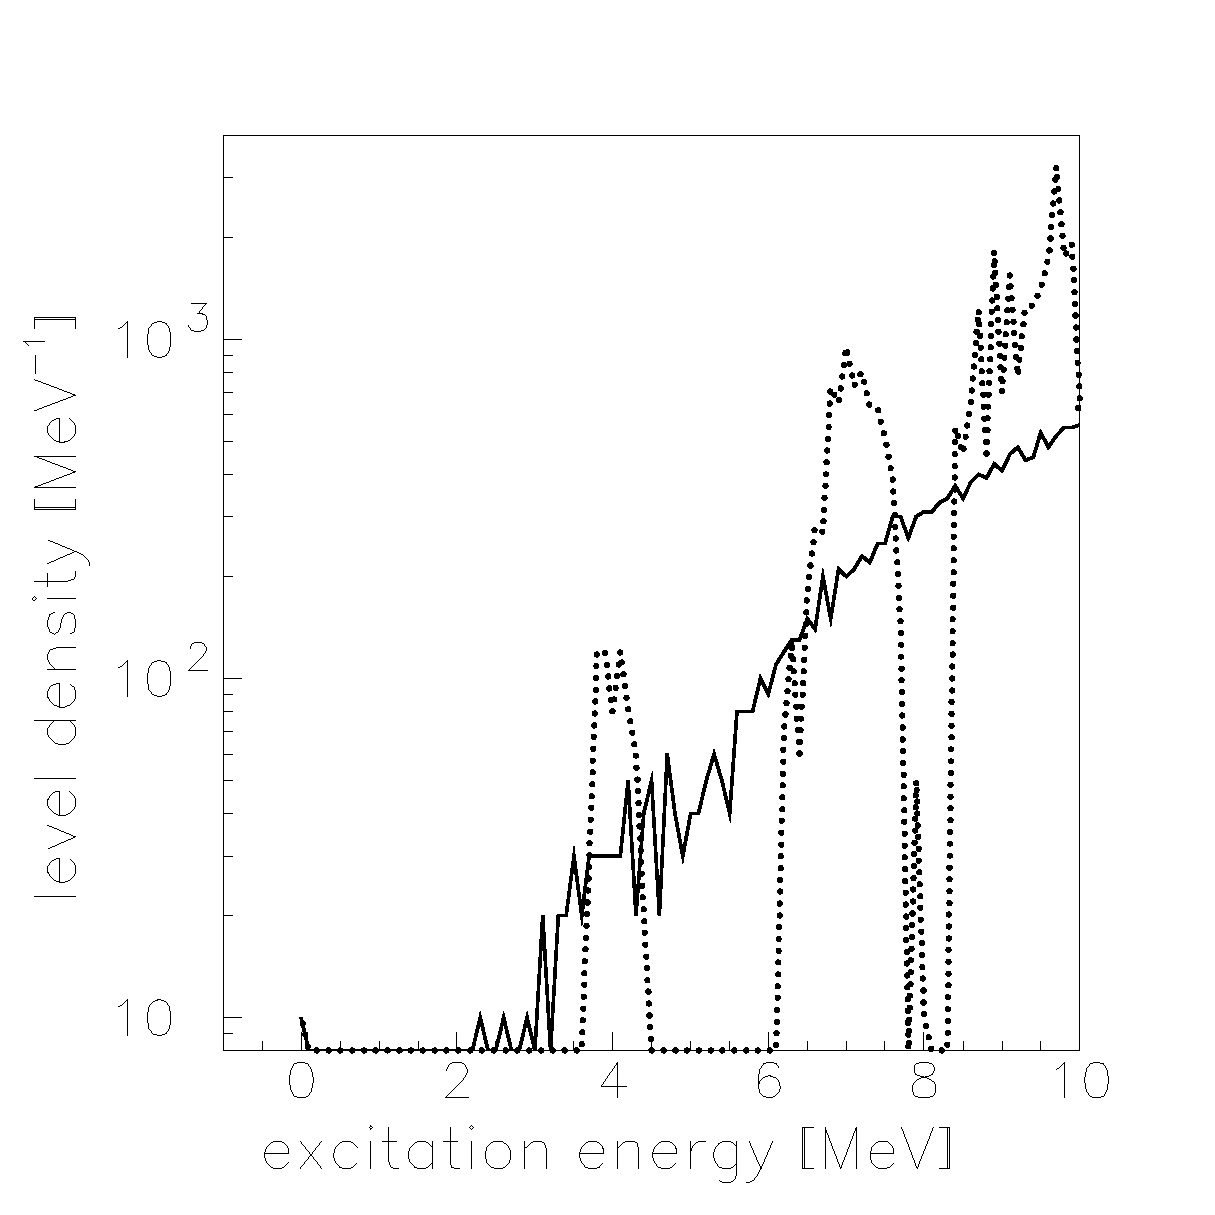
\includegraphics[height=5cm]{fig2b.eps}
\caption{Level density in Fe and Mo isotopes \protect\cite{SA03}. Open and full
symbols follow the same conventions as in Fig.\ \protect\ref{fig:dyyb}. Data 
from counting of discrete levels (jagged line), from neutron resonance spacings
(triangles), from a particle evaporation study (square), and from Fermi-gas 
models (smooth curves) demonstrate the interpolative nature of the results 
obtained by the Oslo method. Arrows point to regions of rapid increase of the 
level density (step structures). Right: calculation of the eigenvalue spectrum 
of a simple model (see Ref.\ \protect\cite{SA03} and text). Dotted line: 
seniority bumps at 4 and 7 MeV due to the breaking of one and two pairs, 
respectively. Solid line: bumps smear out into a plateau-and-step structure due
to the effect of a (random) seniority non-conserving interaction. This 
plateau-and-step structure is reminiscent of similar structures in the 
experimental level density curves from the Oslo method. Thus, our conjecture 
that such structures are due to consecutive breaking of nucleon pairs.}
\label{fig:femotheo}
\end{figure}

\section{Entropy}
\label{sect:entropy}

The entropy $S$ in the microcanonical ensemble is defined as the natural 
logarithm of the multiplicity $\Omega$ of accessible states within the energy 
interval $E$ and $E+\delta E$. In other words, we have 
\begin{equation}
S=k_B\ln\Omega(E).
\end{equation}
The proportionality constant $k_B$ is called Boltzmann's constant and will be 
usually set to unity in the present work, such that the entropy becomes 
dimensionless and temperature will be measured in MeV\@. It is important to 
note that the entropy as function of energy can be defined and measured for 
small and mesoscopic systems as well as for large systems. However, 
fluctuations in level spacings which are typical for small systems will make 
the entropy sensitive to exactly how the energy interval between $E$ and 
$E+\delta E$ is chosen. Thus, the above definition is only useful if $W(E)$ is
a sufficiently smooth function, i.e., for the case that its first derivative, 
the density of levels exists. Consequently, measurements of experimental level 
densities are an important prerequisite for thermodynamical studies of atomic 
nuclei. 

\subsection{Level density and entropy}
\label{sect:spindist}

Unfortunately, the experimentally measured nuclear level density in the present
work does not correspond to a true multiplicity of states. The point is simply
that the level density which enters the formalism of statistical $\gamma$ decay
and which is the result of the Oslo method, does not include the $(2J+1)$ 
degeneracy of magnetic substates. If the spin distribution (or even the average
spin of levels $\langle J\rangle$) at any excitation energy were known, this 
problem could be remedied by simply multiplying an energy-dependent factor
$(2\langle J(E)\rangle+1)$ to the experimental level density. However, little
experimental data exist on the spin distribution. Commonly, a Gaussian 
distribution of spins is assumed with a mean of 
$\langle 2J+1\rangle=\sqrt{2\pi}\,\sigma$ where $\sigma$ is the spin cut-off 
parameter which depends very weakly ($\sigma\propto E^{1/4}$) on excitation 
energy \cite{Be36+GC65}
\begin{equation}
p(J)=\frac{2J+1}{2\,\sigma^2}\,\exp\left(-\frac{\left[J+1/2\right]^2}
{2\,\sigma^2}\right).
\end{equation}
Thus, level density could be converted into multiplicity of states by simply
multiplying a weakly energy-dependent factor $\sqrt{2\pi}\,\sigma$ to it. 
However, some structural transitions of the nucleus like the breaking of 
pairing correlations or shape changes will usually lead to an alteration of the
moment of inertia and might yield a sudden change in the spin distribution of 
levels \cite{JR71}. Therefore, we have decided for the present work that the 
dependence of the spin distribution on energy is too uncertain. Consequently, 
we will present a pseudo-entropy based on level density (without the $(2J+1)$ 
degeneracy) instead of a genuine entropy based on multiplicity. In the case of 
an energy-independent spin distribution the two entropies are equal besides an 
additive constant. All other experimental thermodynamical quantities in this 
work are defined accordingly. When compared to theoretical results like those 
by Y. Alhassid in this book which were obtained by the shell-model Monte Carlo 
method, one has to keep in mind this difference which might lead to potential 
disagreement with our results since the spin distribution of levels is not 
properly taken into account in our work. 

Further, we normalize entropies such that the entropy of even-even nuclei at
ground-state energies becomes zero according to the third law of 
thermodynamics. The same normalization constant is applied to neighboring odd
nuclei which then exhibit a finite entropy for ground-state energies, since the
unpaired nucleon can in general occupy several, nearly degenerate 
single-particle levels.

\subsection{Single-particle entropy}
\label{sect:spe}

As a first step, it is now interesting to compare entropies between neighboring
nuclei. The left panel of Fig.\ \ref{fig:ybentr} shows the entropies of 
$^{170-172}$Yb overlaid on the same plot. It is striking that the entropy 
curves for the even Yb nuclei line up almost perfectly, including their fine 
structures. The entropy of the odd $^{171}$Yb shows a constant offset with 
respect to the entropies of the two even Yb nuclei.\footnote{For a 
constant-temperature level-density model, i.e., a linear entropy model, this is
equivalent to applying a constant energy shift to the level density formula in 
order to describe even and odd nuclei \protect\cite{GH00}.} From this, we can 
already conclude that entropy in atomic nuclei at low energies does not scale 
with the number of nucleons. This is a direct consequence of the strong pairing
interaction between the nucleons. Adopting the language of the Bogoljubov 
transformation, which is useful in describing systems with a strong pairing 
interaction, we can define single-quasiparticle and -quasihole entropies by 
subtracting the entropies of $^{170}$Yb and $^{172}$Yb, respectively, from the 
entropy of $^{171}$Yb. This is shown on the center panel of Fig.\ 
\ref{fig:ybentr}. Since the two entropy differences are equal and independent 
of energy up to the particle separation energy, we can further conclude that 
the relevant nuclear constituents in our region of interest are quasiparticles 
rather then ordinary nucleons. Of course, for temperatures much larger than the
interaction energies which lead to the emergence of quasiparticles, nucleons 
will become the relevant entities again, and nuclear entropy should scale with 
mass number. We estimate the number of quasiparticles at any excitation energy 
by dividing the nuclear entropy by the single-quasihole entropy. This is shown 
on the right panel of Fig.\ \ref{fig:ybentr}. The fine structures in the level 
densities or entropies of $^{172}$Yb and $^{162}$Dy can now be related to 
plateaus in the number of quasiparticles. This supports the interpretation of 
the structures in the level densities as due to the consecutive breaking of 
pairs, since for each broken pair (indicated by a plateau) the number of 
quasiparticles increases roughly by two.

\begin{figure}
\includegraphics[totalheight=5cm,angle=0,bb=45 151 527 651,clip]{fig3a.ps}
\hspace*{0.5cm}
\includegraphics[totalheight=5cm,angle=0,bb=35 148 527 651,clip]{fig3b.ps}
\hspace*{0.5cm}
\includegraphics[totalheight=5cm,angle=0,bb=42 157 527 651,clip]{fig3c.ps}
\caption{Left: entropies of $^{170-172}$Yb superimposed on the same plot. Full 
and open triangles correspond to $^{170}$Yb and $^{172}$Yb, respectively
\protect\cite{AS04}. Center: entropy differences between $^{171}$Yb and 
$^{170}$Yb (single-quasiparticle entropy, full triangles), and between 
$^{171}$Yb and $^{172}$Yb (single-quasihole entropy, open triangles)
\protect\cite{AS04}. Right: Number of quasiparticles in $^{162}$Dy and 
$^{172}$Yb, calculated by scaling the entropies of the two nuclei by the 
respective single-quasihole entropies \protect\cite{GB00}.} 
\label{fig:ybentr}
\end{figure}

Many interesting observations on the single-quasiparticle entropy have been 
made in Ref.\ \cite{GH01}. Most of them rest on the assumption that the level 
density between the two known points from counting of discrete levels and from
neutron resonance spacings can be interpolated by an exponential, the so-called
constant temperature level density $\rho\propto\exp(E/\tau)$, where $\tau$ is 
the constant-temperature parameter. From there, single-quasiparticle entropies
$S_1$ can be calculated at, e.g., 1~MeV and 7~MeV across the nuclear chart for 
mass numbers between 20 and 250. Using this body of data, it has been shown, 
e.g., for the region of deformed rare earth nuclei with $Z=$60--78 and 
$N=$90--110, that $S_1$ at 1~MeV is independent of the ground-state spin of the
involved odd nucleus, and that $S_1$ for quasi-protons equals $1.5\,k_B$, while
$S_1$ for quasi-neutrons equals $1.9\,k_B$. Further, it has been shown that 
$S_1$ around closed shells can become significantly suppressed. This can be 
understood by the fact that a single quasiparticle outside a closed shell has 
very few possibilities for excitations. It is often pinned down in one or a few
single-particle orbitals and cannot give rise to an appreciable amount of 
entropy compared to the neighboring closed-shell nucleus. Such a case 
($^{50,51}$V with $N=$27, 28, where the unpaired quasi-neutron hole is locked 
in the $0f_{7/2}$ orbital) is currently under investigation with the Oslo 
method. 

The importance of the single-quasiparticle entropy can be demonstrated on two 
examples. Let us consider the chemical potential $\mu$ for quasiparticles in 
nuclei.\footnote{This is not the chemical potential for quasiparticles derived 
from Bardeen-Cooper-Schrieffer theory which is equal to zero 
\protect\cite{Mo75}. Rather, we imagine a reaction equilibrium between a Cooper
pair and a couple of unpaired quasiparticles where the breaking of the pair 
costs a certain amount of energy.} It is given by the derivative of the 
Helmholtz free energy $F$ with respect to the quasiparticle number $N$. If the 
chemical potential $\mu$ equals $-\Delta$, i.e., the typical energy cost for 
creating a quasiparticle, the nucleus will be at a transition point between a 
paired and an unpaired nuclear structure. For this to happen, we have to find 
the critical temperature $T_c$ at which $\mu=\partial F/\partial N=-\Delta$. If
we now equate $\partial F/\partial N$ with the ratio of differences 
$\Delta F/\Delta N=(F_{\mathrm{odd}}-F_{\mathrm{even}})/1$, and remember that 
$F_{\mathrm{even}}=E-S\,T$ and $F_{\mathrm{odd}}=F_{\mathrm{even}}-S_1\,T$, we 
find that $T_c=\Delta/S_1$, i.e., the critical temperature is given by the 
ratio of the pairing gap $\Delta$ and the single-quasiparticle entropy $S_1$. 
As a further example, we observe that the relevant Gibbs factor for the 
transition point from a paired to an unpaired nuclear structure is of the order
of $\exp(-\epsilon/T_c)$, where $\epsilon$ is the average single-particle level
spacing of the specific nucleus. This average spacing can be related to the 
Fermi-gas level-density parameter $a$ according to $a=\pi^2/3\,\epsilon$. If we
now express the ratio $\epsilon/T_c$ in terms of the experimentally observable 
quantities $a$, $S_1$, and $\Delta$, we arrive at 
$\epsilon/T_c=\pi^2\,S_1/3\,a\,\Delta$. Under the assumption of a 
constant-temperature level density (see above), the fraction $S_1/\Delta$ can 
also be expressed as $\tau^{-1}$. It has been shown in Ref.\ \cite{GH01} that 
the quantity $\epsilon/T_c\propto S_1/a\,\Delta=0.09$ is constant within 
$\pm 10$\% throughout the nuclear chart where experimental data are available. 
Thus, this second example demonstrates the universality of the pair breaking 
process and establishes the importance of the single-quasiparticle entropy 
$S_1$.

\section{Temperature and caloric curves}
\label{sect:temp}

The generalization of the concept of temperature for a small system is not 
straightforward. Consider the textbook example of a closed macroscopic system 
with total energy $E$ which is divided into one small ($E_1$, $S_1$, 
$\Omega_1$) and one large subsystem ($E_2$, $S_2$, $\Omega_2$) where both 
subsystems can exchange energy with each other. Here, we have not specified the
size of the small subsystem. It can be macroscopic or mesoscopic. We will, 
however, make no \em a priori \rm assumptions for the validity of any familiar 
thermodynamical relation applied to the small system, since we recognize that 
such relations do not necessarily hold in a potentially mesoscopic system. 

The size difference of the two subsystems allows us to expand the entropy of 
the large subsystem into a Taylor series up to first order $S_2(E-E_1)\approx 
S_2(E)-E_1\,\left.\frac{\partial S_2(E^\prime)}{\partial E^\prime}
\right|_{E^\prime=E}$. Since we here consider the large system, we can identify
the first-order term with the familiar $-E_1/T$. Recovering multiplicity 
$\Omega$ from entropy, we arrive at 
$\Omega_2(E-E_1)\approx\Omega_2(E)\,\exp(-E_1/T)$. The probability for 
partitioning the total energy $E$ into $E_1$ and $E_2$ for the two subsystems 
is given by $\Omega_2(E-E_1)\,\Omega_1(E_1)\approx\Omega_2(E)\,\Omega_1(E_1)\,
\exp(-E_1/T)$. The most likely partition of energy is now the one which 
maximizes the expression $\Omega_1(E_1)\,\exp(-E_1/T)$. If the small subsystem 
is macroscopic, this expression will peak very sharply, since it can be shown 
that its width is proportional to $\Delta E/E\propto 1/\sqrt{N}$, where $N$ is 
the number of particles. For mesoscopic systems however, this expression can 
become rather broad and can possibly exhibit several maxima. This case will be 
discussed further on. Here, we would simply point out that maximizing this 
expression corresponds to maximizing its logarithm $S_1-E_1/T=-F_1/T$, or 
minimizing the Helmholtz free energy $F_1$ of the small subsystem. 

The relevance of the above example lies in the fact that it is a model for 
temperature measurements in mesoscopic systems. We adopt here the point of view
that physics, as an experimental science, should only acknowledge observables
which can be measured experimentally. Temperature measurements are carried out
by bringing a thermometer in contact with the system of interest. The contact 
has to allow for energy exchange such that both the system and the thermometer
will attain the same temperature in thermodynamical equilibrium. The 
thermometer has to be characterized, i.e., calibrated to temperature standards 
like the triple point of water, such that its average energy can be readily 
translated into a temperature which is the result of the measuring process. For
a large, macroscopic system, one can imagine a relatively small (but 
macroscopic) thermometer in contact with the system according to the above 
example. The perturbations of the macroscopic system by the thermometer can 
usually be neglected such that the large system can be considered closed 
(microcanonical) if it is so desired. For a mesoscopic system, this concept is 
not feasible since (i) the thermometer taking the place of the small subsystem 
would necessarily need to be a mesoscopic thermometer with all the inherent 
problems of a mesoscopic system which we will discuss later in this work and 
(ii) for the mesoscopic system under consideration which plays the part of the 
large subsystem in our example, we cannot assume \em a priory \rm the validity 
of the expression $\partial S/\partial E=T^{-1}$ which was used in the above 
derivation. Further, it is not guaranteed that the first-order Taylor expansion
of the entropy is sufficient. The correct way of a temperature measurement on a
mesoscopic system is therefore to assume a macroscopic thermometer which plays 
the part of the large subsystem in our example and thus imposes a temperature 
on the small subsystem, i.e., the mesoscopic system under study. With this in 
mind, we reject the notion that the temperature in a closed, i.e., 
microcanonical, mesoscopic system is \em a priori \rm defined by 
$\partial S/\partial E=T^{-1}$, since this definition cannot be verified by any
experimental measurement process. The difficulty lies in the fact that the 
requirement of a microcanonical system precludes energy exchange with any 
macroscopic measurement device (thermometer). 

Experimentally, one has to imagine a cavity heated to a temperature $T$ with a 
nucleus inside. At relevant temperatures, the cavity will emit $\gamma$ rays 
which will be absorbed and re-emitted by the nucleus over time. From repeated
measurements of the energy of the nucleus, an energy distribution for any given
temperature $T$ can be extracted. The probability $p$ to find the nucleus at 
energy $E$ for a given temperature $T$ is given by
\begin{equation}
p(E,T)=\frac{\Omega(E)\,e^{-E/T}}{Z(T)}
\end{equation}
where $\Omega(E)$ is the multiplicity of states (the microcanonical partition 
function) and its Laplace transform 
$Z(T)=\int_0^\infty\Omega(E)\,\exp(-E/T)\,{\mathrm{d}}E$ is the canonical 
partition function. It is interesting to note that equating partial derivatives
of the logarithm of the probability distribution with zero will enable us to 
recover both the microcanonical and canonical definition of the caloric curve 
(the relation between energy and temperature). For example, 
$\partial\ln p/\partial E=0$, i.e., finding extrema of $\ln p$ as function of 
$E$ for a fixed $T$ is equivalent to $\partial S/\partial E=T^{-1}$, and 
$\partial\ln p/\partial T=0$, i.e., finding maxima\footnote{The extrema of 
$\ln p$ as function of $T$ are maxima, since it can be shown that the second
derivative of $\ln p$ with respect to $T$ evaluated at the extrema equals 
$-(\langle E^2\rangle-\langle E\rangle^2)/T^4=-C_V/T^2$ which is always 
negative.} of $\ln p$ as function of $T$ for a fixed $E$ corresponds to 
$E=T^2\,\partial\ln Z(T)/\partial T$.\footnote{It is also worth noting that the
canonical caloric curve gives the average energy $\langle E\rangle$ of the 
distribution $p(E,T)$ for a given temperature $T$.} This means that when we 
plot the probability $p(E,T)$ as a contour plot with $E$ on the horizontal axis
and $T$ on the vertical axis, the microcanonical caloric curve is given by the 
ensemble of points where the contour lines have horizontal tangents, while the 
canonical caloric curve is given by the ensemble of points where the contours 
have vertical tangents. This is demonstrated on the lower left panel of Fig.\ 
\ref{fig:cal}.

\begin{figure}
\includegraphics[totalheight=8cm,angle=0,bb=138 147 408 655,clip]{fig4a.ps}
\hspace*{3cm}
\includegraphics[totalheight=8cm,angle=0,bb=65 28 442 619,clip]{fig4b.ps}
\caption{Upper left: model of bimodal entropy $S(E)$. Lower left: probability
distribution $p(E,T)$ derived from the bimodal entropy model. The ensembles of 
points where contour lines (solid lines) of $p(E,T)$ exhibit horizontal and 
vertical tangents equal the microcanonical (dashed) and canonical (dotted) 
caloric curves, respectively. The dash-dotted line depicts our new concept of a
'mesoscopic' caloric curve (see text and Ref.\ \protect\cite{SG03} for more 
details). Right: microcanonical (data points) and canonical (lines) caloric 
curves derived from experimental level density data on $^{162}$Dy, $^{166}$Er, 
and $^{172}$Yb \protect\cite{MB99}. The two caloric curves show qualitative 
agreement with aspects of the model on the left.} 
\label{fig:cal}
\end{figure}

The special interest for mesoscopic systems lies in the fact that the 
experimentally measurable probability $p(E,T)$ can become broad. As function of
$E$, it can exhibit more than one maximum (at which point it will also contain 
one or more local minima), and its most likely value (the global maximum) will 
in general not coincide with the average value of the distribution. The 
physical reason for this is simply the mesoscopic character of the system. The 
situation is indeed not unlike quantum mechanics with its distributions of the 
position and the momentum of an object. These distributions are connected with 
each other by a Fourier transformation which gives rise to a minimum combined 
width (or uncertainty) of the two. This is reflected by Heisenberg's 
uncertainty relation. However, this minimum uncertainty becomes only 
appreciable in small (quantal) systems. In thermodynamics, the microcanonical 
(control parameter $E$) and canonical (control parameter $T$) partition 
functions are connected with each other by the mathematically similar Laplace 
transformation. Thus, it should not be surprising that thermodynamical 
quantities derived from these partition functions will exhibit distributions 
with finite widths (or uncertainties). These widths will have an appreciable 
impact on the thermodynamics of mesoscopic systems. We will explore some of the
consequences in the following. Most importantly, we will concentrate on the 
caloric curve, i.e., the supposedly one-to-one relationship between the 
temperature and the energy of a system. Obviously, such a relationship will be 
subject to uncertainties in the presence of wide distributions of the 
probability $p(E,T)$.

One of the simplest distribution $p(E,T)$ is created by a bimodal entropy model
shown on the upper left panel of Fig.~\ref{fig:cal}. This model contains a 
locally convex entropy. The microcanonical caloric curve, connecting all 
contours of $p(E,T)$ with horizontal tangents becomes multivalued for some 
temperatures. It is obvious that for these temperatures the microcanonical 
caloric curve not only picks up the global maxima of $p(E,T)$ as function of 
$E$, but also all local maxima and minima. In other words, for some instances, 
the microcanonical caloric curve describes the energy distribution $p(E,T)$ by 
its locally least probable value. Such a description is unphysical and we were 
justified to reject the \em a priori \rm applicability of 
$\partial S/\partial E=T^{-1}$ for mesoscopic systems. The failure of the 
microcanonical caloric curve has a one-to-one correspondence with the 
appearance of microcanonical negative heat capacities. We therefore also reject
the notion of the reality of such negative heat capacities. We conclude that 
negative heat capacities are artifacts which arise due to the wrongful 
introduction, i.e., not based on a measurement process, of the concept of 
temperature to a closed, mesoscopic system.

The concept of caloric curves is discussed in further detail in Ref.\ 
\cite{SG03}. Some of the conclusions are listed in the remainder of this 
section. For once, shortcomings of the microcanonical caloric curve 
$\partial S/\partial E=T^{-1}$ are not limited to artificial negative heat 
capacities. An entropy model which is not only locally convex, but also locally
decreasing can, e.g., lead to artificially negative temperatures. Also, the 
canonical caloric curve has shortcomings. It can be shown that it, too, for a 
given temperature $T$ can produce values of $E$ for which $p(E,T)$ assumes a 
local minimum. It can go even so far that this local minimum of $p(E,T)$ equals
zero, i.e., that the probability of finding the system under study at its 
average value $\langle E\rangle$ is vanishing. Furthermore, the average nature 
of the canonical caloric curve (due to the Laplace transformation involved in 
calculating the canonical partition function) glosses too much over potentially
true structural changes of mesoscopic systems which might manifest themselves 
exactly by the presence of a locally convex entropy.

The nature of the geometric constructs to obtain caloric curves from contour 
plots of $p(E,T)$ illuminates the fact that for a given energy $E$, the 
microcanonical caloric curve tends to give larger values of $T$ than the 
canonical caloric curve. This is seen in experiment as well. For demonstration,
on the right panel of Fig.\ \ref{fig:cal}, we show microcanonical (data points)
and canonical (lines) caloric curves \cite{MB99} derived from the same set of 
level density data.\footnote{In order to calculate the canonical caloric curve,
the experimental level density had to be extrapolated by a Fermi-gas expression
$\rho\propto\exp(2\sqrt{a\,E})/E^{3/2}$ in order to evaluate the canonical 
partition function at sufficiently high temperatures.} The inverse derivative 
involved in calculating the microcanonical caloric curve emphasizes the 
underlying structures in the level densities curves which are thought to be due
to the breaking of pairs.\footnote{For different isotopes these structures in 
the level densities do not appear at the same excitation energies. However, 
these fluctuations in energies are expected from isotope to isotope much in the
same way as binding energies of different isotopes can fluctuate as it is 
discussed in the contributions of O. Bohigas and F. Leboeuf to this book.} 
However, in light of the discussion above, we would like not to attach any 
physical relevance to the microcanonical caloric curve in terms of an actual 
thermodynamical temperature or in terms of the resulting negative heat 
capacities. Our example merely illustrates the facts that (i) microcanonical 
and canonical caloric curves are in general different for mesoscopic systems, 
the latter one producing in average smaller values of the temperature for a 
given energy and that (ii) locally convex entropies exist in nature for 
mesoscopic systems and they can lead to unphysical claims of negative heat 
capacities or temperatures by a naive application of microcanonical 
thermodynamics. 

Finally, we have proposed \cite{SG03} a different geometrical construct for a 
'mesoscopic' caloric curve which avoids some of the shortfalls of both the 
microcanonical and canonical caloric curve. Our construct for the 'mesoscopic'
caloric curve is also a geometric one and requires that it has to intersect the
contour curves of $p(E,T)$ perpendicularly, and that it has to coincide with 
both the microcanonical and canonical caloric curve in the thermodynamical 
limit. It is obtained by solving the differential equation
\begin{equation}
\left(\frac{E}{T^2}-\frac{\partial}{\partial T}\,\ln\,Z(T)\right){\mathrm{d}}E=
\left(\frac{\partial}{\partial E}\,\ln\,W(E)-\frac{1}{T}\right){\mathrm{d}}T
\end{equation}
under the condition that the resulting curve always lies in between the 
microcanonical and canonical caloric curve. This 'mesoscopic' caloric curve 
avoids negative heat capacities and negative temperatures, it follows more 
closely the global maximum of $p(E,T)$ as function of $E$ than the canonical 
caloric curve, thus, reflecting more of the possible structural changes in the 
nucleus. It avoids areas of low probability $p$ to a larger extent (but not
completely) than either the microcanonical and canonical caloric curves. 
However, one has to still keep in mind that a one-to-one correspondence of 
energy and temperature as it is expressed by the concept of a caloric curve, is
at best an approximation in the presence of wide distributions $p(E,T)$ which 
are typical for mesoscopic systems. In general, the presence of broad or 
multi-peaked distributions usually indicates that average or approximate 
thermodynamic concepts like the caloric curve are applied at an energy scale at
which the system is still inherently discrete and thus, the application of such
concepts might not always be useful.

\section{Phase transitions}
\label{sect:phasetrans}

We have in the past applied several different methods to investigate a possible
phase transition from a paired phase to an unpaired phase of the nucleus with
increasing excitation energy or temperature. Here, we would like to point out 
once more that while there is no doubt that the observed structures in the 
level density are manifestations of the breaking of nucleon Cooper pairs, only 
by applying the language of thermodynamics can we investigate if the phenomenon
under study corresponds to an actual phase transition in a mesoscopic system 
reminiscent a phase transition of macroscopic systems with Fermionic pairing.

\subsection{Microcanonical heat capacity}
\label{sect:miccv}

In Ref.\ \cite{MG01}, we have tried to apply the microcanonical caloric curve 
and the observation of a negative microcanonical heat capacity as a criterion  
for the existence of a first-order phase transition. In light of the discussion
in Sect.\ \ref{sect:temp} it should not be surprising that the results were 
physically unsatisfactory. Typical small wriggles in the entropy would imply a 
series of first-order phase transitions for the gradual depairing process in 
atomic nuclei which is an unattractive result. Furthermore, the long-range 
nature of pairing correlations also prohibits the interpretation of locally 
convex entropies in terms of geometrical surface entropy \cite{Gr97}. Thus, we 
reject to equate the observation of negative microcanonical heat capacities 
with the existence of a first-order phase transition.

\subsection{Linearized Helmholtz free energy}
\label{sect:fc}

In Ref.\ \cite{GC03}, we define the linearized Helmholtz free energy as 
$F(E)=E-T\,S(E)$ where we avoid any introduction of a caloric curve by keeping 
the temperature $T$ constant. Finding the global minimum of $F(E)$ for a given 
temperature $T$ will actually provide an alternative definition of a caloric 
curve. The critical value $T_c$ for a potential phase transition is defined for
the case in which $F_c(E)=E-T_c\,S(E)$ exhibits a double-minimum structure 
where both minima are equally deep (see left panel of Fig.\ 
\ref{fig:phasetrans}).\footnote{A double-minimum structure is typically caused 
by a locally convex entropy.} Assuming the first pair breaks at the energy 
$2\,\Delta$ and creates an entropy in the order of two single-quasiparticle 
entropies $2S_1$, we can again derive from the equality of the two minima at 
$E=0$ and $E=2\,\Delta$ the relation $T_c=\Delta/S_1$ which we have discussed 
in Sect.\ \ref{sect:spe} and which yields a critical temperature for the 
breaking of the first pair in the order of 0.45~MeV\@. The barrier height 
between the two minima for even-even rare earth nuclei is in the order of 
0.5~MeV\@. The dependence of the barrier height on the system size governs the 
existence and order of a possible phase transition 
\cite{LK90+LK91}.\footnote{This is different from Sect.\ 
\protect\ref{sect:miccv} where the criterion for a first-order phase transition
was the mere existence of a barrier in the linearized Helmholtz free energy, or
equivalently, the presence of a locally convex entropy.} Unfortunately, there 
is no trend discernible from our limited experimental data. 

For odd rare earth nuclei and for the breaking of further pairs in even-even 
rare earth nuclei no appreciable barrier in the linearized Helmholtz free 
energy appears. Rather, for a slightly higher critical temperature of 0.52~MeV,
a broad, flat minimum stretching over $\sim 4$~MeV in excitation energy 
emerges, reflecting roughly a constant-temperature level density. The higher 
critical temperature for this phenomenon is attributed to the Pauli blocking 
effect of the unpaired quasiparticles which somewhat increases the cost in 
energy to break up pairs into further quasiparticles. It seems that this effect
dominates slightly over the weakening of pairing correlations (and consequently
the reducing of the cost in energy to break further pairs) in the presence of 
already unpaired quasiparticles. In other words, while the quenching of pairing
correlations reduces the energy to break a pair, Pauli blocking prevents the 
two newly created quasiparticles to acquire the full single-quasiparticle 
entropy unless some more energy is supplied to the system to counteract the 
effect of Pauli blocking. The two effects combined work at smearing out in 
energy the process of depairing in the presence of unpaired quasiparticles. 
Thus, we can understand that using the method of the linearized Helmholtz free 
energy, a possible phase transition is most likely attached to the breaking of 
the first pair in even-even nuclei, while the smearing in energy of the 
depairing process in the presence of unpaired quasiparticles prohibits the 
emergence of significant structures in $F_c(E)$ for higher energies and 
therefore does not suggest a phase transition for these cases.

\begin{figure}
\includegraphics[totalheight=5cm,angle=0,bb=51 156 528 651,clip]{fig5a.ps}
\hspace*{1.5cm}
\includegraphics[totalheight=5cm,angle=0,bb=151 141 402 608,clip]{fig5b.ps}
\hspace*{1.5cm}
\includegraphics[totalheight=5cm,angle=0,bb=219 422 414 625,clip]{fig5c.ps}
\caption{Linearized Helmholtz free energy (data points with error bars) for 
$^{162}$Dy at the critical temperature for the breaking of the first pair 
(upper left), for the breaking of further pairs (center left) and for the 
breaking of pairs in $^{161}$Dy (lower left) \protect\cite{GC03}. Canonical 
heat capacities (solid lines) in $^{171}$Yb (upper center) and $^{172}$Yb 
(lower center), estimates for a non-interacting Fermi gas (dashed lines), and 
fits to data using a constant-temperature level-density model for the canonical
heat capacity (dash-dotted lines) \protect\cite{SB01}. The dash-dotted vertical
lines indicate the extracted critical temperatures. Right panel: zeros of the 
canonical partition functions in the complex temperature plane for $^{162}$Dy 
(represented by poles of the heat capacity) \protect\cite{Bo01}. More details 
about all panels are given in the text.} 
\label{fig:phasetrans}
\end{figure}

\subsection{Canonical heat capacity}

The canonical heat capacity shows local enhancements around $T\sim 0.5$~MeV 
over expectations for a non-interacting Fermi gas (see center panels of Fig.\ 
\ref{fig:phasetrans}). These enhancements are larger for even-even than for odd
rare earth nuclei and the extracted critical temperatures are slightly higher 
for odd than for even-even rare earth nuclei \cite{SB01}. The critical 
temperatures have been obtained by a fit of the canonical heat capacity of a 
constant-temperature level-density model to the data for the first 400~keV in 
temperature. This method avoids uncertainties due to the necessary 
extrapolation of the level density by a Fermi-gas expression in order to 
evaluate the canonical partition function at higher temperatures ($>0.5$~MeV). 
Also, this method can be shown to yield necessarily very similar values for the
critical temperatures \cite{GC03} as the method using the linearized Helmholtz 
free energy. The heat capacity curves resemble washed-out step structures. A 
discontinuity of the heat capacity in a macroscopic system indicates a 
second-order phase transition according to the Ehrenfest classification which 
is indeed observed in the case of a transition of a paired Fermion system like 
a low-temperature superconductor or superfluid $^3$He to their normal phases. 
Thus, the experimentally observed local enhancement of the heat capacity might 
indicate a corresponding second-order phase transition in a mesoscopic system 
like the atomic nucleus. For small superconducting particles, a gradual change 
(as function of decreasing size) from a step structure to a local enhancement 
in the heat capacity has been observed and modeled successfully \cite{LA93}. 
For atomic nuclei within the shell-model Monte Carlo method, Y. Alhassid has 
shown the emergence of local enhancements in the canonical heat capacity due to
a gradual breakdown of pairing correlations (see his contribution to this 
book). However, a direct one-to-one comparison between our results and the 
results by Y. Alhassid has to take into account the missing $m$-degeneracy in 
the present data (see Sect.\ \ref{sect:spindist}). A drawback of the canonical 
heat capacity is the large smoothing introduced by the Laplace transformation 
in calculating the canonical partition function which prevents us from 
obtaining separated structures in the canonical heat capacity corresponding to 
the breaking of consecutive pairs. The introduction of the 'mesoscopic' caloric
curve (and its derivative, the 'mesoscopic' heat capacity) might improve this 
situation somewhat, on the other hand, the 'mesoscopic' heat capacity cannot be
simply related to energy fluctuations between the heat bath and the mesoscopic 
system under study, thus the physical interpretation of the 'mesoscopic' heat 
capacity is still somewhat unclear.

\subsection{Zeros of canonical partition function in complex temperature plane}

Borrmann \sl et al.\ \rm have shown that the zeros of the canonical partition 
function in the complex temperature plane can be used to classify phase 
transitions in mesoscopic systems using a scheme which reduces to the Ehrenfest
classification scheme in the thermodynamical limit \cite{BM00}. The advantage 
of extending the canonical partition function into the complex temperature 
plane lies in the fact that the complete thermodynamical information of the 
system becomes available. While on the real temperature axis, only heavily 
smoothed (averaged) thermodynamical quantities can be investigated, the fact 
that the inverse Laplace transformation which is needed to recover the 
multiplicity of states has to be performed along a line parallel to the 
imaginary temperature axis illuminates the importance of including complex 
temperatures. Unfortunately, the experimental level density data are too noisy 
\cite{Bo01} to produce meaningful distributions of zeros of the canonical 
partition function (see right panel of Fig.\ \ref{fig:phasetrans}). Zeros in 
the complex temperature plane based on microscopic model calculations have 
until now suffered from limitations of the model space \cite{BD01}. We have 
developed a more schematic model \cite{GH01,GH01b,SG02b} including a sufficient
number of particles in an infinite model space which contains the two most 
important physics processes contributing to the depairing process: the 
weakening of pairing correlations which decreases the cost of energy for 
breaking pairs in the presence of unpaired quasiparticles and the Pauli 
blocking, which decreases the amount of entropy created by pair breaking in the
presence of unpaired quasiparticles. We have shown that our model reproduces 
well the experimental level densities (using the saddle-point approximation for
the inverse Laplace transformation \cite{GH01b}), odd-even effects in the 
canonical entropy \cite{GH01} which have been observed in data and microscopic 
calculations \cite{GB00}, the experimentally observed local enhancements in the
canonical heat capacity \cite{GH01b} (including the odd-even effect), the 
experimentally observed skewness of the distribution $p(E,T)$ as function of 
energy for a given temperature \cite{GB03}, and the gradual decrease of the 
effective pairing-gap parameter $\Delta$ with temperature \cite{SG02b}. These 
positive results give us confidence that our model also might reflect the 
correct distribution of zeros of the canonical partition function in the 
complex temperature plane \cite{SG02b}. Our model calculations show two phase 
transitions. One is a first-order phase transition from an interacting Fermi 
gas to an interacting diluted phase where Pauli blocking becomes negligible. 
This phase transition shows no odd-even dependence and is only relevant for 
mesoscopic systems since the critical temperature will approach infinity in the
thermodynamical limit of $N\rightarrow\infty$ number of particles. For atomic 
nuclei in particular, however, it is not relevant since it takes place at high 
temperatures for which other factors like nuclear binding energies become 
important which are not included in our model. The second transition is the 
pairing phase transition. Its critical temperature is independent of the number
of particles (when keeping the other model parameters constant) and gives 
somewhat higher values for odd than for even nuclei due to the slight dominance
of Pauli blocking over the quenching of pairing correlations in the presence of
unpaired quasiparticles. Applying a general scaling of model parameters with 
mass number $A$, we could show that a second-order pairing phase transition 
exists for even-even nuclei with masses $A>100$ with an $A^{2/3}$ dependence of
the inverse critical temperature. This dependence can be understood in terms of
the scaling of $\Delta$ and $S_1$ with mass number in the region of deformed 
rare earth nuclei. As discussed in Sects.\ \ref{sect:spe} and \ref{sect:fc}, 
the ratio of these two quantities equals the critical temperature 
$T_c=\Delta/S_1$. For odd nuclei, the pairing phase transition has been 
determined to be of higher-than-second order within the model.

\section{Conclusion}

Starting from an experimental method to measure level densities up to the 
particle separation energy we first demonstrated that fine structures in these 
level densities are due to the consecutive breaking of nucleon Cooper pairs. 
Our goal was to investigate this transition in the language of thermodynamics 
in order to find out whether it can be described as a mesoscopic phase 
transition reminiscent of the breakdown of bulk low-temperature 
superconductivity or superfluidity of $^3$He where pairing of Fermions plays an
important role, too. In Sect.\ \ref{sect:entropy}, we investigated the entropy 
of the system and showed that the relevant constituents of the nucleus at our 
low energies are quasiparticles with excitation-energy independent 
single-quasiparticle entropy. We illustrated the relevance of the 
single-quasiparticle entropy which allowed us (i) to extract the number of 
excited quasiparticles with excitation energy, (ii) to derive a critical 
temperature for the depairing process, and (iii) to demonstrate the 
universality of the pair-breaking process across the nuclear chart. 

In Sect.\ \ref{sect:temp}, we introduced the concept of temperature to 
mesoscopic systems by proposing a measurement process. This led us to a 
rejection of the microcanonical definition $\partial S/\partial E=T^{-1}$ of 
the temperature in mesoscopic systems and consequently to the rejection of the 
reality of negative heat capacities. We showed that the probability 
distribution $p(E,T)=\Omega(E)\,\exp(-E/T)/Z(T)$ is of great importance for the
discussion of thermodynamics of mesoscopic systems and that the definitions of 
both the microcanonical and canonical caloric curves can be obtained from 
$p(E,T)$ by geometric constructions. Typical large widths of $p(E,T)$ for 
mesoscopic systems lead to uncertainties in approximate thermodynamical 
concepts like the caloric curve which replaces projections of the distribution 
$p(E,T)$ by special values like their extrema or averages. Applying such 
approximate concepts to mesoscopic systems at an energy scale for which the 
system under study is inherently discrete, will not always yield useful 
results. We have proposed a 'mesoscopic' caloric curve also based on a 
geometric construct on $p(E,T)$ which avoids some, but not all of the 
shortcomings of the microcanonical and canonical caloric curves.

In Sect.\ \ref{sect:phasetrans}, we have applied several different ways to 
investigate a potential phase transitions from a paired to an unpaired phase in
atomic nuclei. The first method, based on the linearized Helmholtz free energy 
avoids any complication due to the definition of caloric curves. However, it 
could not be demonstrated that the barrier in the Helmholtz free energy 
increases sufficiently with mass number in order to indicate a true 
thermodynamic phase transition. The second method, based on the derivative of 
the canonical caloric curve, i.e., the canonical heat capacity, shows 
structures reminiscent of a second-order phase transition. The finite size of 
atomic nuclei smoothes out what in the bulk is supposedly a step-like structure
of the heat capacity to a gradual transition within a finite temperature range.
The third method, based on the zeros of the canonical partition function in the
complex temperature plane seems to be the most promising method. It avoids any 
reference to caloric curves and makes use of the full information contained in 
the canonical partition function by extending it to complex temperatures. 
However, until now, the existence of a pairing phase transition in atomic 
nuclei could only be demonstrated within a schematic nuclear model for heavy 
$(A>100)$ nuclei. Thus, the existence of a true phase transition in a rigorous 
thermodynamical sense from a paired to an unpaired phase in atomic nuclei is 
still an unsolved problem in nuclear structure which is certainly worth further
attention. A common result from our various investigations is that in general 
for odd nuclei weaker signals for a potential phase transition are obtained 
than for even nuclei, and that Pauli blocking (winning the competition against 
the weakening of pairing correlations in the presence of already unpaired 
quasiparticles) is responsible for slightly higher critical temperatures for 
the depairing process in odd nuclei than in even nuclei.

\begin{theacknowledgments}
Part of this work was performed under the auspices of the U.S. Department of 
Energy by the University of California, Lawrence Livermore National Laboratory
under Contract No.\ W-7405-ENG-48\@. Part of this research is was sponsored by 
the National Nuclear Security Administration under the Stewardship Science
Academic Alliances program through DOE research Grants No.\ DE-FG03-03-NA00074 
and No.\ DE-FG03-03-NA00076\@. E.A. acknowledges support by a U.S. Department 
of Energy Grant No.\ DE-FG02-97-ER41042\@. Financial support from the Norwegian
Research Council (NFR) is gratefully acknowledged. We would like to thank Peter
Borrmann and his collaborators for preparing the right panel of Fig.\ 
\ref{fig:phasetrans}. A.S. would like to thank Vladimir Zelevinsky for many 
interesting discussions and for carefully reading the manuscript.
\end{theacknowledgments}

\bibliographystyle{aipproc}

\begin{thebibliography}{9}
\bibitem{MH00}Luciano Maiani \sl et al.\rm, CERN seminar, Geneva, Switzerland, 
Feb.\ 10, 2000, and CERN Bulletin 07/00, Feb.\ 14, 2000. 
\bibitem{PM95}J. Pochodzalla \sl et al.\rm, Phys.\ Rev.\ Lett.\ \bf 75\rm, 1040
(1995).
\bibitem{Er60}T. Ericson, Adv.\ Phys.\ \bf 9\rm, 425 (1960).
\bibitem{KA98}Dimitri Kusnezov, Y. Alhassid, and K. A. Snover, Phys.\ Rev.\ 
Lett.\ \bf 81\rm, 542 (1998).
\bibitem{MB99}E. Melby \sl et al.\rm, Phys.\ Rev.\ Lett.\ \bf 83\rm, 3150 
(1999).
\bibitem{SW72}Mitsuo Sano and Masamiti Wakai, Prog.\ Theor.\ Phys.\ \bf 48\rm, 
160 (1972).
\bibitem{RN84}J. Rekstad \sl et al.\rm, Nucl.\ Phys.\ \bf A417\rm, 376 (1984).
\bibitem{Br55+Ax62}D. M. Brink, PhD thesis, Oxford University, 1955; P. Axel, 
Phys.\ Rev.\ \bf 126\rm, 671 (1962).
\bibitem{GB03}M. Guttormsen \sl et al.\rm, Phys.\ Rev.\ C \bf 68\rm, 064306
(2003).
\bibitem{AS04}U. Agvaanluvsan \sl et al.\rm, Phys.\ Rev.\ C \bf 70\rm, 054611
(2004).
\bibitem{SG00}A. Schiller, M. Guttormsen, E. Melby, J. Rekstad, and S. Siem, 
Phys.\ Rev.\ C \bf 61\rm, 044324 (2000).
\bibitem{GT96}M. Guttormsen, T. S. Tveter, L. Bergholt, F. Ingebretsen, and J. 
Rekstad, Nucl.\ Instrum.\ Methods Phys.\ Res.\ A \bf 374\rm, 371 (1996).
\bibitem{GR87}M. Guttormsen, T. Rams{\o}y, and J. Rekstad, Nucl.\ Instrum.\
Methods Phys.\ Res.\ A \bf 255\rm, 518 (1987).
\bibitem{HB95}L. Henden, L. Bergholt, M. Guttormsen, J. Rekstad, and T. S. 
Tveter, Nucl.\ Phys.\ \bf A589\rm, 249 (1995).
\bibitem{SB00}A. Schiller \sl et al.\rm, Nucl.\ Instrum.\ Methods Phys.\ Res.\ 
A \bf 447\rm, 498 (2000).
\bibitem{BA73}G. A. Bartholomew, E. D. Earle, A. J. Ferguson, J. W. Knowles, 
and M. A. Lone, Adv.\ Nucl.\ Phys.\ \bf 7\rm, 229 (1973).
\bibitem{SA03}A. Schiller \sl et al.\rm, Phys.\ Rev.\ C \bf 68\rm, 054326 
(2003).
\bibitem{MG01}E. Melby \sl et al.\rm, Phys.\ Rev.\ C \bf 63\rm, 044309 (2001).
\bibitem{SG02}S. Siem \sl et al.\rm, Phys.\ Rev.\ C \bf 65\rm, 044318 (2002).
\bibitem{GM03}M. Guttormsen \sl et al.\, J. Phys.\ G \bf 29\rm, 263 (2003).
\bibitem{VG01}A. Voinov \sl et al.\rm, Phys.\ Rev.\ C \bf 63\rm, 044313 (2001).
\bibitem{VA04}A. Voinov \sl et al.\rm, Phys.\ Rev.\ Lett.\ \bf 93\rm, 142504
(2004).
\bibitem{TB95}T. S. Tveter, L. Bergholt, M. Guttormsen, E. Melby, and J. 
Rekstad, Phys.\ Rev.\ Lett.\ \bf 77\rm, 2404 (1995).
\bibitem{GB00}M. Guttormsen \sl et al.\rm, Phys.\ Rev.\ C \bf 62\rm, 024306 
(2000).
\bibitem{DJ03}D. J. Dean and M. Hjorth-Jensen, Rev.\ Mod.\ Phys.\ \bf 75\rm, 
607 (2003).
\bibitem{Be36+GC65}H. Bethe, Phys.\ Rev.\ \bf 50\rm, 332 (1936); A. Gilbert and
A. G. W. Cameron, Can.\ J. Phys.\ \bf 43\rm, 1446
(1965).
\bibitem{JR71}A. Johnson, H. Ryde, and J. Sztarkier, Phys.\ Lett.\ \bf 34B\rm, 
605 (1971).
\bibitem{GH01}M. Guttormsen \sl et al.\rm, Phys.\ Rev.\ C \bf 63\rm, 044301 
(2001).
\bibitem{GH00}M. Guttormsen \sl et al.\rm, Phys.\ Rev.\ C \bf 61\rm, 067302
(2000).
\bibitem{Mo75}L. G. Moretto, Nucl.\ Phys.\ \bf A243\rm, 77 (1975).
\bibitem{SG03}A. Schiller, M. Guttormsen, M. Hjorth-Jensen, J. Rekstad, and S.
Siem, preprint nucl-th/0306082.
\bibitem{Gr97}D. H. E. Gross, Phys.\ Rep.\ \bf 279\rm, 119 (1997).
\bibitem{GC03}M. Guttormsen \sl et al.\rm, Phys.\ Rev.\ C \bf 68\rm, 034311 
(2003).
\bibitem{LK90+LK91}Jooyoung Lee and J. M. Kosterlitz, Phys.\ Rev.\ Lett.\ \bf 
65\rm, 137 (1990), and Phys.\ Rev.\ B \bf 43\rm, 3265 (1991).
\bibitem{SB01}A. Schiller \sl et al.\rm, Phys.\ Rev.\ C \bf 63\rm, 021306(R) 
(2001).
\bibitem{Bo01}Peter Borrmann, private communication.
\bibitem{LA93}Bent Lauritzen, Andrea Anselmino, P. F. Bortignon, and Ricardo 
Broglia, Ann.\ Phys.\ (NY) \bf 223\rm, 216 (1993). 
\bibitem{BM00}Peter Borrmann, Oliver M\"{u}lken, and Jens Harting, Phys.\ Rev.\
Lett.\ \bf 84\rm, 3511 (2000).
\bibitem{BD01}A. Beli\'{c}, D. J. Dean, and M. Hjorth-Jensen, preprint 
cond-mat/0104138.
\bibitem{GH01b}M. Guttormsen \sl et al.\rm, Phys.\ Rev.\ C \bf 64\rm, 034319 
(2001).
\bibitem{SG02b}A. Schiller, M. Guttormsen, M. Hjorth-Jensen, J. Rekstad, and S.
Siem, Phys.\ Rev.\ C \bf 66\rm, 024322 (2002).
\end{thebibliography}

\end{document}

\endinput
